\documentclass{standalone}
\usepackage{tikz}
\usepackage{ctex,siunitx}
\setCJKmainfont{Noto Serif CJK SC}
\usepackage{tkz-euclide}
\usepackage{amsmath}
\usetikzlibrary{patterns, calc}
\usetikzlibrary {decorations.pathmorphing, decorations.pathreplacing, decorations.shapes,}
\begin{document}
\small
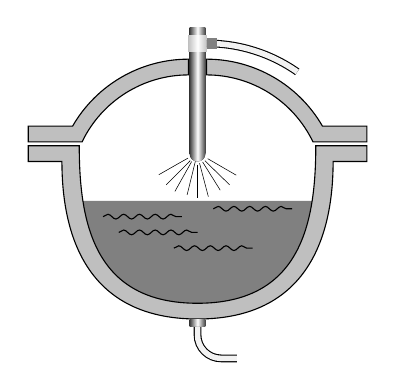
\begin{tikzpicture}[>=latex,scale=1.0]
  % \useasboundingbox(-2,-2.2)rectangle(2,1.5);
  \draw[fill=lightgray](-2.15,0.85)--++(0,-0.2)--++(0.6841,0)arc(154.321:90:1.5)--++(0,0.2)arc(90:150:1.7)--cycle;
  \draw[fill=lightgray](2.15,0.85)--++(0,-0.2)--++(-0.6841,0)arc(25.679:90:1.5)--++(0,0.2)arc(90:30:1.7)--cycle;
  \fill[left color=darkgray,right color=darkgray,middle color=white](0,0.5)circle(0.1);
  \fill[left color=darkgray,right color=darkgray,middle color=white](-0.1,0.5)rectangle(0.1,2.1);
  \fill[left color=lightgray,right color=lightgray,middle color=white](-0.12,1.8)rectangle(0.12,2.0);
  \draw[double=lightgray!20,double distance=2pt](0.12,1.9)arc(90:55:2.0);
  \fill[gray](0.12,1.83)rectangle(0.25,1.97);
  \fill[gray](-1.590,-0.1)--(-1.207,-1.066)--( 0.000,-1.600)--( 1.207,-1.066)--( 1.590,-0.1)--cycle;
  \draw[fill=lightgray](-1.502, 0.600)..controls(-1.502,-0.413)and(-1.294,-1.400)..( 0.000,-1.400)..controls( 1.294,-1.400)and( 1.502,-0.413)..( 1.502, 0.600)--( 2.150, 0.600)--( 2.150, 0.400)--( 1.722, 0.400)..controls( 1.722,-0.431)and( 1.476,-1.600)..( 0.000,-1.600)..controls(-1.476,-1.600)and(-1.722,-0.431)..(-1.722, 0.400)--(-2.150, 0.400)--(-2.150, 0.600)--cycle;
  \fill[left color=darkgray,right color=darkgray,middle color=white](-0.1,-1.6)rectangle(0.1,-1.7);
  \draw[double=lightgray!20,double distance=2pt](0,-1.7)--(0,-1.8)arc(180:270:0.3)--++(0.2,0);
  \foreach \x in {-150,-135,...,-30}
  {
    \draw[very thin]([shift=(\x:0.1+0.05*rnd)]0,0.5)--++(\x:0.4+0.05*rnd);
  }
  \foreach \x/\y in {-1/-0.5,0.2/-0.2,-0.3/-0.7,-1.2/-0.3}
  {\draw[decorate,decoration={snake,amplitude=0.3mm,segment length=2mm}](\x,\y)--++(1.0,0);}
  \end{tikzpicture}
\end{document}